\documentclass[journal,12pt,twocolumn]{IEEEtran}

\usepackage{setspace}
\usepackage{gensymb}
\singlespacing
\usepackage[cmex10]{amsmath}

\usepackage{amsthm}

\usepackage{mathrsfs}
\usepackage{txfonts}
\usepackage{stfloats}
\usepackage{bm}
\usepackage{cite}
\usepackage{cases}
\usepackage{subfig}

\usepackage{longtable}
\usepackage{multirow}

\usepackage{enumitem}
\usepackage{mathtools}
\usepackage{steinmetz}
\usepackage{tikz}
\usepackage{circuitikz}
\usepackage{verbatim}
\usepackage{tfrupee}
\usepackage[breaklinks=true]{hyperref}
\usepackage{graphicx}
\usepackage{tkz-euclide}

\usetikzlibrary{calc,math}
\usepackage{listings}
    \usepackage{color}                                            %%
    \usepackage{array}                                            %%
    \usepackage{longtable}                                        %%
    \usepackage{calc}                                             %%
    \usepackage{multirow}                                         %%
    \usepackage{hhline}                                           %%
    \usepackage{ifthen}                                           %%
    \usepackage{lscape}     
\usepackage{multicol}
\usepackage{chngcntr}
\usepackage{textcomp}
\usepackage{float}
\restylefloat{table}

\DeclareMathOperator*{\Res}{Res}

\renewcommand\thesection{\arabic{section}}
\renewcommand\thesubsection{\thesection.\arabic{subsection}}
\renewcommand\thesubsubsection{\thesubsection.\arabic{subsubsection}}

\renewcommand\thesectiondis{\arabic{section}}
\renewcommand\thesubsectiondis{\thesectiondis.\arabic{subsection}}
\renewcommand\thesubsubsectiondis{\thesubsectiondis.\arabic{subsubsection}}


\hyphenation{op-tical net-works semi-conduc-tor}
\def\inputGnumericTable{}                                 %%

\lstset{
%language=C,
frame=single, 
breaklines=true,
columns=fullflexible
}
\begin{document}

\newcommand{\BEQA}{\begin{eqnarray}}
        \newcommand{\EEQA}{\end{eqnarray}}
\newcommand{\define}{\stackrel{\triangle}{=}}
\bibliographystyle{IEEEtran}
\raggedbottom
\setlength{\parindent}{0pt}
\providecommand{\mbf}{\mathbf}
\providecommand{\pr}[1]{\ensuremath{\Pr\left(#1\right)}}
\providecommand{\qfunc}[1]{\ensuremath{Q\left(#1\right)}}
\providecommand{\sbrak}[1]{\ensuremath{{}\left[#1\right]}}
\providecommand{\lsbrak}[1]{\ensuremath{{}\left[#1\right.}}
    \providecommand{\rsbrak}[1]{\ensuremath{{}\left.#1\right]}}
    \providecommand{\brak}[1]{\ensuremath{\left(#1\right)}}
    \providecommand{\lbrak}[1]{\ensuremath{\left(#1\right.}}
    \providecommand{\rbrak}[1]{\ensuremath{\left.#1\right)}}
    \providecommand{\cbrak}[1]{\ensuremath{\left\{#1\right\}}}
    \providecommand{\lcbrak}[1]{\ensuremath{\left\{#1\right.}}
    \providecommand{\rcbrak}[1]{\ensuremath{\left.#1\right\}}}
    \theoremstyle{remark}
    \newtheorem{rem}{Remark}
    \newcommand{\sgn}{\mathop{\mathrm{sgn}}}
    \providecommand{\abs}[1]{\vert#1\vert}
    \providecommand{\res}[1]{\Res\displaylimits_{#1}}
    \providecommand{\norm}[1]{\lVert#1\rVert}
    %\providecommand{\norm}[1]{\lVert#1\rVert}
    \providecommand{\mtx}[1]{\mathbf{#1}}
    \providecommand{\mean}[1]{E[#1]}
    \providecommand{\fourier}{\overset{\mathcal{F}}{ \rightleftharpoons}}
    %\providecommand{\hilbert}{\overset{\mathcal{H}}{ \rightleftharpoons}}
    \providecommand{\system}{\overset{\mathcal{H}}{ \longleftrightarrow}}
    %\newcommand{\solution}[2]{\textbf{Solution:}{#1}}
    \newcommand{\solution}{\noindent \textbf{Solution: }}
    \newcommand{\cosec}{\,\text{cosec}\,}
    \newcommand{\comb}[2]{{}^{#1}\mathrm{C}_{#2}}
    \providecommand{\dec}[2]{\ensuremath{\overset{#1}{\underset{#2}{\gtrless}}}}
    \newcommand{\myvec}[1]{\ensuremath{\begin{pmatrix}#1\end{pmatrix}}}
    \newcommand{\mydet}[1]{\ensuremath{\begin{vmatrix}#1\end{vmatrix}}}
    \numberwithin{equation}{subsection}
    \makeatletter
    \@addtoreset{figure}{problem}
    \makeatother
    \let\StandardTheFigure\thefigure
    \let\vec\mathbf
    \renewcommand{\thefigure}{\theproblem}
    \def\putbox#1#2#3{\makebox[0in][l]{\makebox[#1][l]{}\raisebox{\baselineskip}[0in][0in]{\raisebox{#2}[0in][0in]{#3}}}}
    \def\rightbox#1{\makebox[0in][r]{#1}}
    \def\centbox#1{\makebox[0in]{#1}}
    \def\topbox#1{\raisebox{-\baselineskip}[0in][0in]{#1}}
    \def\midbox#1{\raisebox{-0.5\baselineskip}[0in][0in]{#1}}
    \vspace{3cm}
    \title{AI1103 Assignment-8}
    \author{SRIVATSAN T - CS20BTECH11062}
    \maketitle
    \newpage
    \bigskip
    \renewcommand{\thefigure}{\theenumi}
    \renewcommand{\thetable}{\theenumi}
    Download all python codes from
    \begin{lstlisting}
https://github.com/CS20BTECH11062/AI1103/tree/main/Assignment-8/codes
\end{lstlisting}
    %
    and latex-tikz codes from
    %
    \begin{lstlisting}
https://github.com/CS20BTECH11062/AI1103/tree/main/Assignment-8/Assignment-8.tex
\end{lstlisting}
    \section*{QUESTION\\(UGC MATH (mathA) June 2017 Q.52)}
    X and Y are independent random variables each having the density
    \begin{align}
        f(t) = \displaystyle\frac{1}{\pi} \frac{1}{1+{t}^2} -\infty < t < +\infty
    \end{align}
    Then the density function of $\displaystyle\frac{X+Y}{3}$ for \\$-\infty <$ t $< +\infty$ is\bigskip
        \begin{enumerate}\itemsep0.5cm
            \item $\displaystyle\frac{6}{\pi} \frac{1}{4+9{t}^2}$
            \item $\displaystyle\frac{6}{\pi} \frac{1}{9+4{t}^2}$
            \item $\displaystyle\frac{3}{\pi} \frac{1}{1+9{t}^2}$
            \item $\displaystyle\frac{3}{\pi} \frac{1}{9+{t}^2}$
        \end{enumerate}
        \section*{SOLUTION}
        Let us consider the random variables $\displaystyle\frac{X}{3}$ and $\displaystyle\frac{Y}{3}$.\\[0.3cm]
We know that if a random variable M has a probability density $f_M(x)$, then the probability density of kM is
\begin{align}
    f_{kM}\brak{x} = \frac{1}{\abs{k}} f_M\brak{\frac{x}{\abs{k}}}
\end{align}
Let the probability densities of $\displaystyle\frac{X}{3}$ and $\displaystyle\frac{Y}{3}$ be $f_{1}\brak{x}$ and $f_{2}\brak{y}$.
\begin{align}
    f_{1}\brak{x} = & \hspace{0.2cm} 3\times f\brak{3x}                                                                \\
    =               & \hspace{0.2cm} \displaystyle\frac{3}{\pi} \frac{1}{1+9{x}^2} \hspace{0.2cm}-\infty < x < +\infty \\[0.3cm]
    f_{2}\brak{y} = & \hspace{0.2cm} 3\times f\brak{3y}                                                                \\
    =               & \hspace{0.2cm} \displaystyle\frac{3}{\pi} \frac{1}{1+9{y}^2} \hspace{0.2cm}-\infty < y < +\infty
\end{align}
Then the probability density of $\displaystyle\frac{X}{3}$ + $\displaystyle\frac{Y}{3}$ is the\\[0.1cm]convolution of probability densities of $\displaystyle\frac{X}{3}$ and $\displaystyle\frac{Y}{3}$.
\begin{align}
    f_{Z}\brak{z} = & \int_{-\infty}^{+\infty} f_{1}\brak{z-y} f_{2}\brak{y} dy                                                                              \\[0.3cm]
    =               & \int_{-\infty}^{+\infty} \displaystyle\frac{3}{\pi}\frac{1}{1+9{\brak{z-y}^2}}\times\displaystyle\frac{3}{\pi} \frac{1}{1+9{{y}^2}} dy \\[0.3cm]
    =               & \frac{9}{{\pi}^2} \int_{-\infty}^{+\infty} \frac{1}{1+9{\brak{z-y}^2}}\times\frac{1}{1+9{{y}^2}} dy                                    \\[0.3cm]
    =               & \frac{9}{{\pi}^2}\times\frac{2\pi}{3} \displaystyle\frac{1}{4 + 9{z}^2}                                                                \\[0.3cm]
    =               & \frac{6}{\pi} \displaystyle\frac{1}{4 + 9{z}^2}\hspace{0.2cm}-\infty < z < +\infty
\end{align}
\begin{align}
    f_{Z}\brak{t} = \frac{6}{\pi} \displaystyle\frac{1}{4 + 9{t}^2}\hspace{0.2cm}-\infty < t < +\infty
\end{align}
\begin{center}
    Correct Option : 1
\end{center}
\begin{figure}[H]
    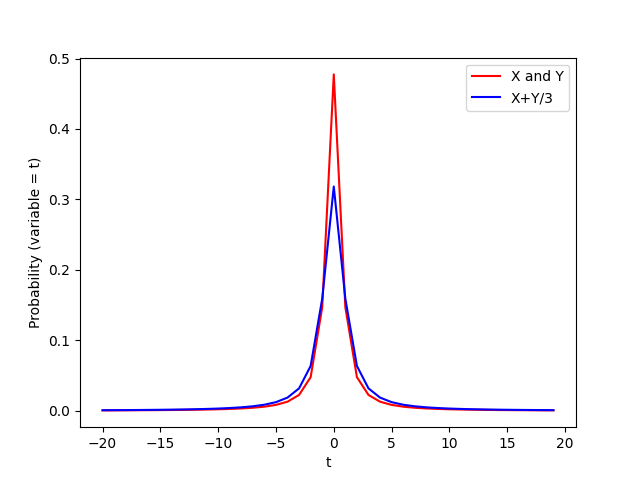
\includegraphics[width = \columnwidth]{Assignment-8.png}
    \caption{Grphs showing initial and convoluted probability densities.Area under both the curves = 1}
\end{figure}
\end{document}